\documentclass[10pt, compress]{beamer}

\usetheme[numbering=fraction, sectionpage=none, progressbar=frametitle]{m}
\usepackage{booktabs}
\usepackage{array}
\usepackage{listings}
\usepackage{graphicx}
\usepackage[brazilian]{babel}
\usepackage[scale=2]{ccicons}
\usepackage{url}
\usepackage{relsize}
\usepackage{courier}

\usepackage{pgfplots}
\usepgfplotslibrary{dateplot}

\lstset{basicstyle=\footnotesize\ttfamily,breaklines=true}
\renewcommand*{\UrlFont}{\ttfamily\smaller\relax}

\graphicspath{{./img/}}

\title{Autotuning usando Busca Estocástica Local
e Paralelismo na linguagem Julia}
\subtitle{}
\author{\footnotesize Pedro Bruel \\ {\scriptsize phrb@ime.usp.br} \\[0.2cm]
Alfredo Goldman \\{\scriptsize gold@ime.usp.br} }
\institute{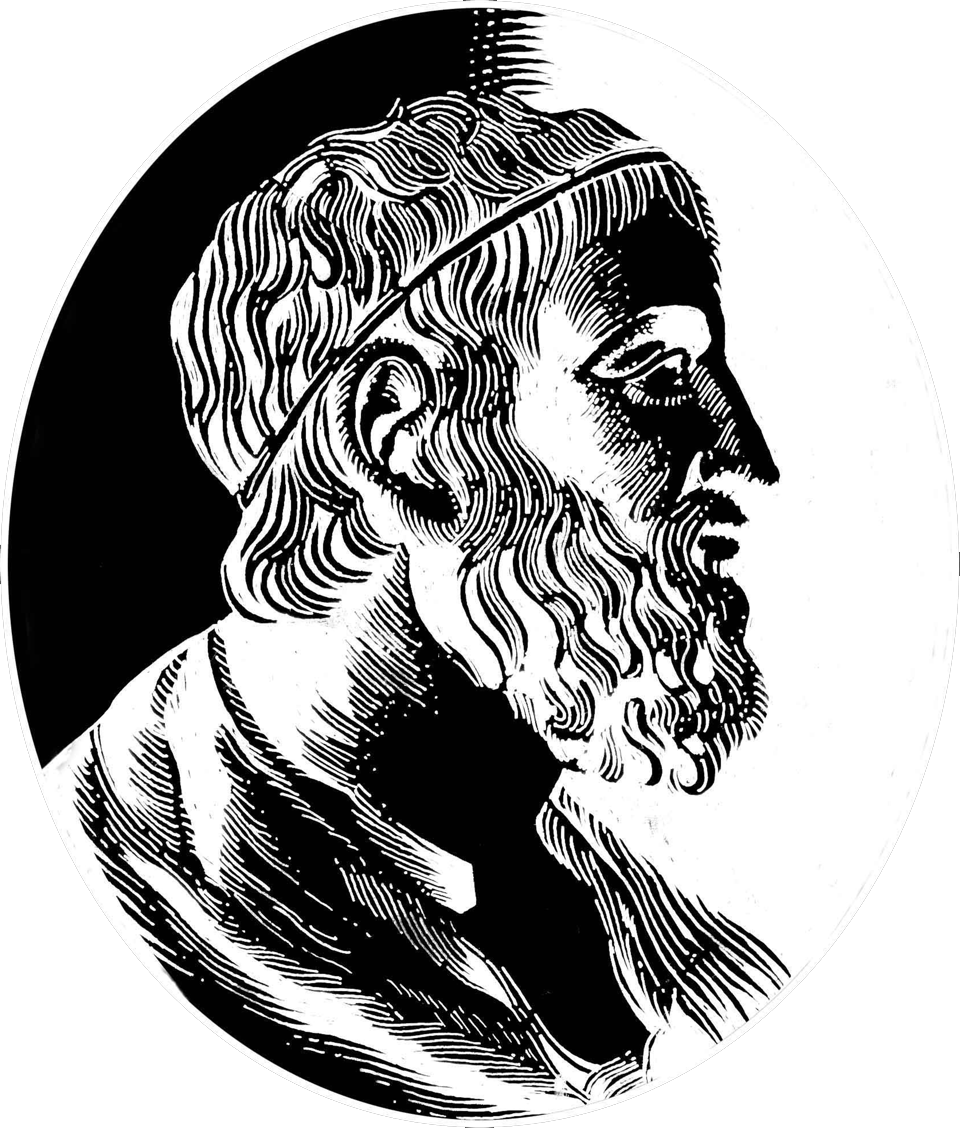
\includegraphics[height=2cm]{imelogo}\\[0.2cm] Instituto de Matemática e Estatística \\ Universidade de São Paulo}
\date{\scriptsize 29 de Setembro de 2015}

\begin{document}

\maketitle

\begin{frame}
    \frametitle{Roteiro}
    \setbeamertemplate{section in toc}[sections numbered]
    \tableofcontents[hideallsubsections]
\end{frame}

\section{Motivação e Perguntas de Pesquisa}

\begin{frame}[fragile]
    \frametitle{Motivação}
    \begin{itemize}
        \item \alert{Modelos de programação} paralela e distribuída
        \item \alert{Arquiteturas} multi-core e co-processadores
            \pause
        \item \alert{Autotuning} com programação paralela e distribuída
            \pause
        \item Problemas \alert{computacionalmente difíceis}
            \pause
        \item Estudar o desempenho da \alert{Busca Estocástica Local}
    \end{itemize}
\end{frame}

\begin{frame}[fragile]
    \frametitle{Motivação}
    \begin{figure}[H]
        \centering
        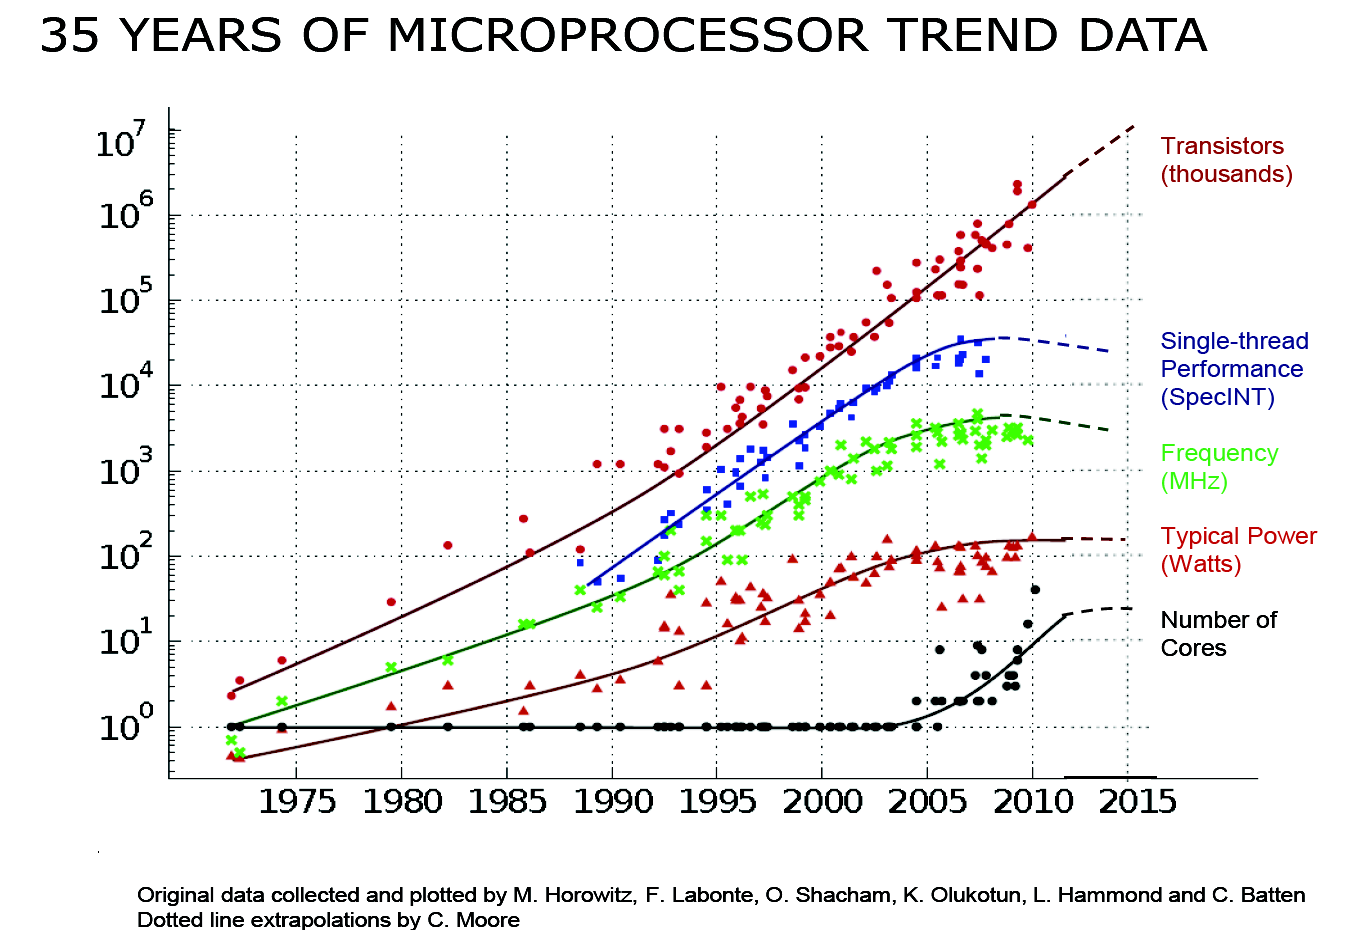
\includegraphics[width=1\textwidth]{35years}
    \end{figure}%
    \let\thefootnote\relax\footnotetext{Karl Rupp: \url{http://goo.gl/WLdveJ}}
\end{frame}

\begin{frame}[fragile]
    \frametitle{Motivação}
    \begin{figure}[H]
        \centering
        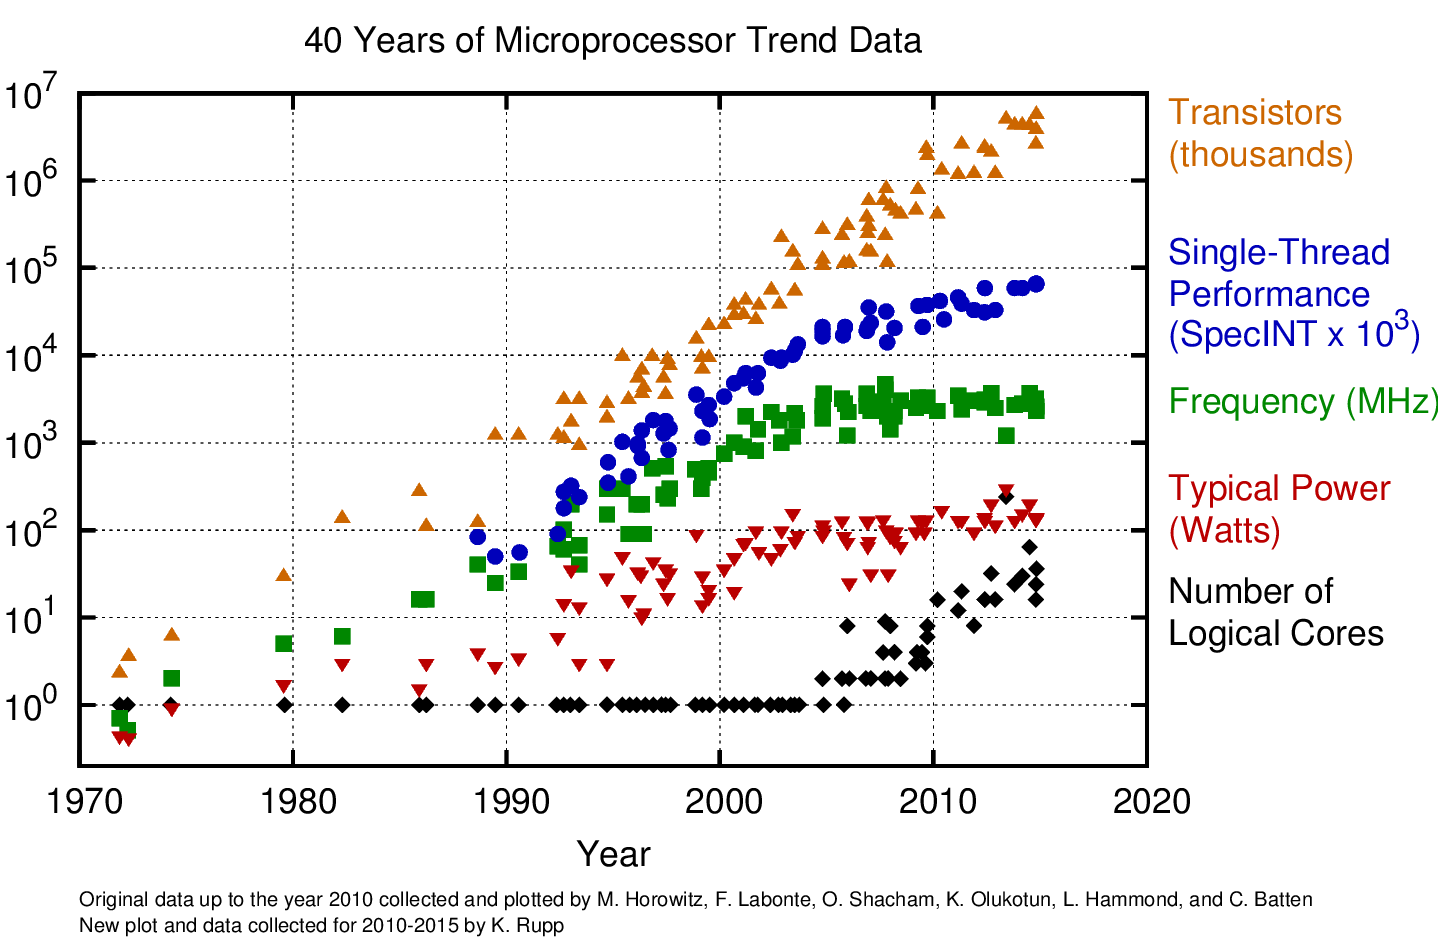
\includegraphics[width=1\textwidth]{40years}
    \end{figure}%
    \let\thefootnote\relax\footnotetext{Karl Rupp: \url{http://goo.gl/WLdveJ}}
\end{frame}

\begin{frame}[fragile]
    \frametitle{Perguntas de Pesquisa}
    Visão geral:
    \begin{itemize}
        \item \alert{RQ0}: Como e quando aplicar técnicas de
            autotuning a problemas difíceis e arquiteturas heterogêneas?
            \pause
        \item \alert{RQ1}: Técnicas de busca estocástica apresentam
            alguma vantagem em relação a outras técnicas de autotuning?
            \pause
        \item \alert{RQ2\textbf{a}}: Como utilizar programação paralela e
            distribuída para melhorar o desempenho de autotuners?
        \item \alert{RQ2\textbf{b}}: Para quais domínios de problema isso é
            vantajoso?
            \pause
        \item \alert{RQ3}: Como aproveitar medições de desempenho obtidas
            em arquiteturas diferentes da arquitetura alvo?
    \end{itemize}
\end{frame}

\begin{frame}[fragile]
    \frametitle{Perguntas de Pesquisa}
    Com este trabalho em andamento, gostaríamos de avançar em
    direção a responder:
    \begin{itemize}
        \item \alert{RQ1}: Técnicas de busca estocástica apresentam
            alguma vantagem em relação a outras técnicas de autotuning?
        \item \alert{RQ2\textbf{a}}: Como utilizar programação paralela e
            distribuída para melhorar o desempenho de autotuners?
        \item \alert{RQ2\textbf{b}}: Para quais domínios de problema isso é
            vantajoso?
    \end{itemize}
\end{frame}

\section{Autotuning \& OpenTuner}

\begin{frame}[fragile]
    \frametitle{Autotuning}
    \begin{columns}
        \column{0.5\textwidth}
        \centering
        Configurações e Otimizações
        \column{0.5\textwidth}
        \centering
        Espaço de Busca
    \end{columns}
    \begin{figure}[H]
        \centering
        \includegraphics[width=1\textwidth]{autotuning}
    \end{figure}
\end{frame}

\subsection{OpenTuner}

\begin{frame}[fragile]
    \frametitle{OpenTuner}
    \begin{figure}[H]
        \centering
        
\includegraphics[width=.34\textwidth]{opentuner-logo}
    \end{figure}%
    \begin{itemize}
        \item \alert{Arcabouço} para autotuning
        \item \alert{Independente} de domínio
            \pause
        \item \alert{Conjuntos} de técnicas de busca
        \item \alert{Compartilhamento} de resultados entre técnicas
            \pause
        \item Execução \alert{sequencial}
    \end{itemize}
    \let\thefootnote\relax\footnotetext{Código sob Licença MIT: \href{http://github.com/jansel/opentuner}{\tt github.com/jansel/opentuner}}
\end{frame}

\begin{frame}[fragile]
    \frametitle{OpenTuner}
    \begin{figure}[H]
        \centering
        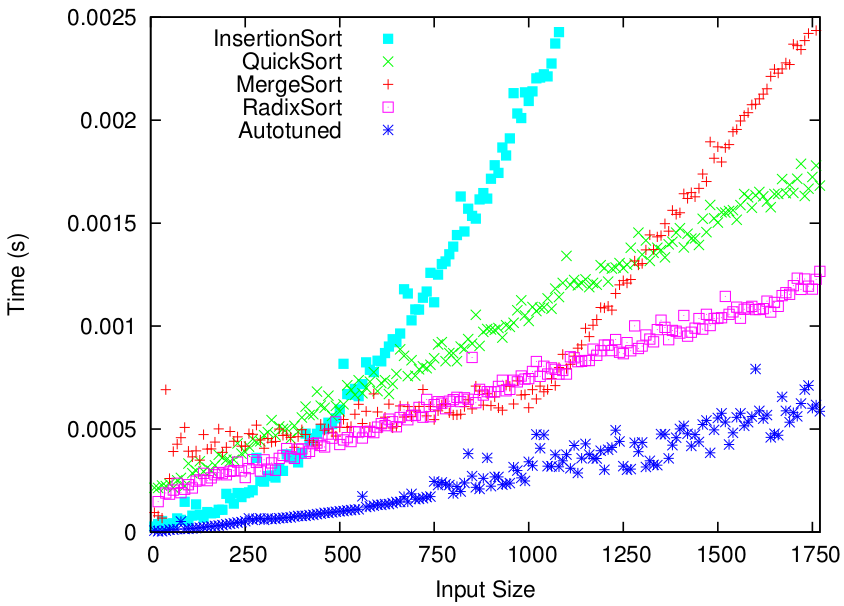
\includegraphics[width=.8\textwidth]{sorting}
        \caption{Otimizando combinações de algoritmos recursivos de ordenação}
    \end{figure}%
    \let\thefootnote\relax\footnotetext{Ansel, Jason, et al. "Opentuner: An extensible framework for program autotuning." Proceedings of the 23rd ICPAC. ACM, 2014.}
\end{frame}

\begin{frame}[fragile]
    \frametitle{OpenTuner}
    Trabalho com OpenTuner em andamento (disponível no \alert{GitHub}):
    \begin{itemize}
        \item Computação Distribuída (\alert{Google Compute Engine}):
            \href{https://github.com/phrb/gce\_autotuning\_example}{\tt phrb/gce\_autotuning\_example}

            \href{https://github.com/phrb/measurement\_client}{\tt phrb/measurement\_client}

            \href{https://github.com/phrb/gce\_interface}{\tt phrb/gce\_interface}

            \href{https://github.com/phrb/measurement-server}{\tt phr/measurement-server}
            \pause
        \item Parâmetros de compilação em GPUs (\alert{CUDA}):
            \href{https://github.com/phrb/gpu-autotuning}{\tt phrb/gpu-autotuning}
            \pause
        \item Resolvedores de \alert{SAT} e \alert{TSP}:

            \href{https://github.com/phrb/sat-opentuner}{\tt phrb/sat-opentuner}

            \href{https://github.com/phrb/stochasticsearch-docs}{\tt phrb/stochasticsearch-docs}
    \end{itemize}
\end{frame}

\section{Busca Estocástica Local}

\begin{frame}[fragile]
    \frametitle{Busca Estocástica Local}
    \begin{columns}
        \column{0.4\textwidth}
        \centering
        \begin{figure}[h]
            \centering
            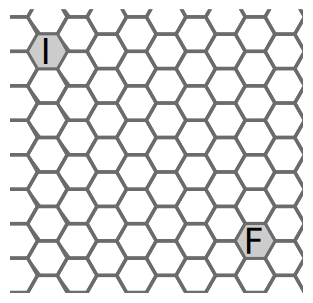
\includegraphics[width=1\textwidth]{hex_map}
        \end{figure}
        \column{0.4\textwidth}
        \centering
        \begin{figure}[h]
            \centering
            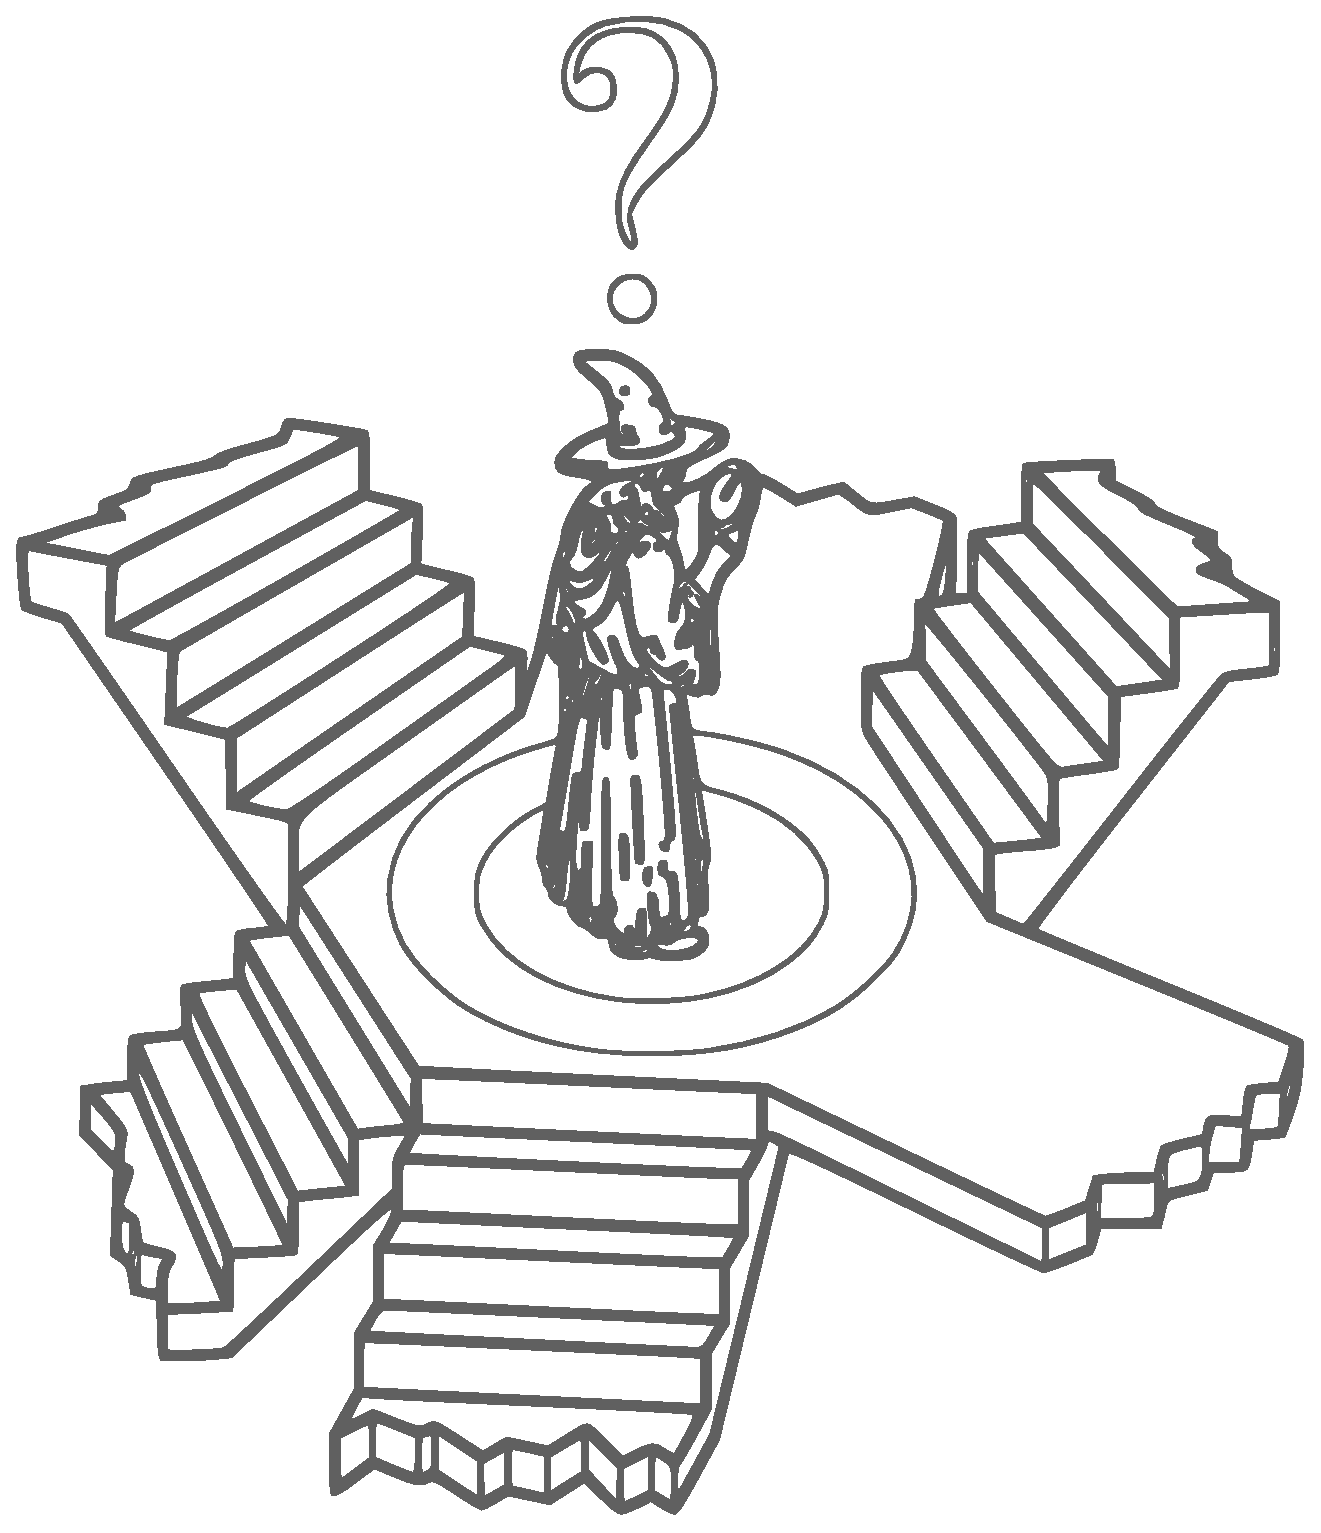
\includegraphics[width=1\textwidth]{gandalfsearch}
        \end{figure}
    \end{columns}
    \let\thefootnote\relax\footnotetext{Adaptado de: Hoos, Holger H., and Thomas Stützle.
        \emph{Stochastic local search: Foundations \& applications.} Elsevier, 2004.}
\end{frame}

\begin{frame}[fragile]
    \frametitle{Busca Estocástica Local}
    Os algoritmos de Busca Estocástica Local consistem de
    \alert{heurísticas} para a exploração de um espaço de busca.
    \pause
    \begin{itemize}
        \item Naturalmente \alert{paralelas} e \alert{distribuídas}
        \item Podem ser \alert{combinadas} para gerar novas heurísticas
            \pause
        \item \alert{Fáceis} de implementar
            \pause
        \item \alert{Estado da Arte}\footnotemark[1]\footnotemark[2] na solução
            de \alert{alguns tipos} de instâncias de problemas computacionalmente
            difíceis
    \end{itemize}
    \footnotetext[1]{Hutter, Frank, et al. \emph{ParamILS: an automatic
        algorithm configuration framework.} Journal of Artificial
        Intelligence Research. 2009.}
    \footnotetext[2]{Dubois-Lacoste, et al. \emph{On the Empirical Scaling
        Behaviour of State-of-the-art Local Search Algorithms for the Euclidean
        TSP.} Proceedings of the 2015 GECCO. ACM, 2015.}
\end{frame}

\begin{frame}[fragile]
    \frametitle{Composição}
    Alguns \alert{blocos de construção}:
    \begin{itemize}
        \item First Improvement
        \item Best Improvement
        \item Probabilistic Improvement
        \item Greedy Construction
        \item Random Walk
    \end{itemize}
            \pause
    Exemplo de \alert{composição}:

    $ProbabilisticImprovement(Temperatura) \rightarrow SimulatedAnnealing$
\end{frame}

\begin{frame}[fragile]
    \frametitle{Busca Estocástica Local}
    Principais referências:

    \textbf{[1]} Hoos, Holger H., and Thomas Stützle.
    \emph{Stochastic local search: Foundations \& applications.} Elsevier, 2004.
            \pause

    \textbf{[2]} Hoos, Holger H., and Thomas Stützle. \emph{Stochastic Local Search Algorithms: An Overview.}
    Springer Handbook of Computational Intelligence. Springer Berlin Heidelberg, 2015. 1085-1105.
            \pause

    \textbf{[3]} Hutter, Frank, et al. \emph{ParamILS: an automatic
    algorithm configuration framework.} Journal of Artificial
    Intelligence Research 36.1 (2009): 267-306.
\end{frame}

\section{StochasticSearch.jl}

\begin{frame}[fragile]
    \frametitle{StochasticSearch.jl: Justificativa}
    Por que uma nova implementação?

    OpenTuner:
    \begin{itemize}
        \item Permite \alert{pouco controle} do fluxo de execução
            \pause
        \item Python: \alert{Global Interpreter Lock}
            \pause
        \item Busca e Medições \alert{sequenciais}
            \pause
        \item Não é fácil de \alert{paralelizar}
    \end{itemize}
    \pause
    Outros motivos:
    \begin{itemize}
        \item Estudar a \alert{composição} e o \alert{desempenho} de técnicas
            de Busca Estocástica Local
            \pause
        \item Tentativa de \alert{reproduzir} resultados
    \end{itemize}
\end{frame}

\begin{frame}[fragile]
    \frametitle{StochasticSearch.jl: Julia}
    \begin{figure}[H]
        \centering
        
\includegraphics[width=.24\textwidth]{julialogo}
    \end{figure}%
    Por que em Julia?
    \begin{itemize}
        \item Linguagem de \alert{alto nível}
        \item Programação \alert{concorrente}, \alert{paralela} e \alert{distribuída}
            \pause
        \item Ótimo \alert{desempenho}
            \pause
        \item É um brinquedo \alert{novo}
        \item Comunidade bastante \alert{ativa} (\textbf{v0.4.x-stable}, \textbf{v0.5-dev})
    \end{itemize}
    \let\thefootnote\relax\footnotetext{Código sob Licença MIT: \href{http://github.com/JuliaLang/julia}{\tt github.com/JuliaLang/julia}}
\end{frame}

\begin{frame}[fragile]
    \frametitle{StochasticSearch.jl: Julia}
    Comparações de desempenho relativo à linguagem \alert{C}:
    \begin{figure}[H]
        \centering
        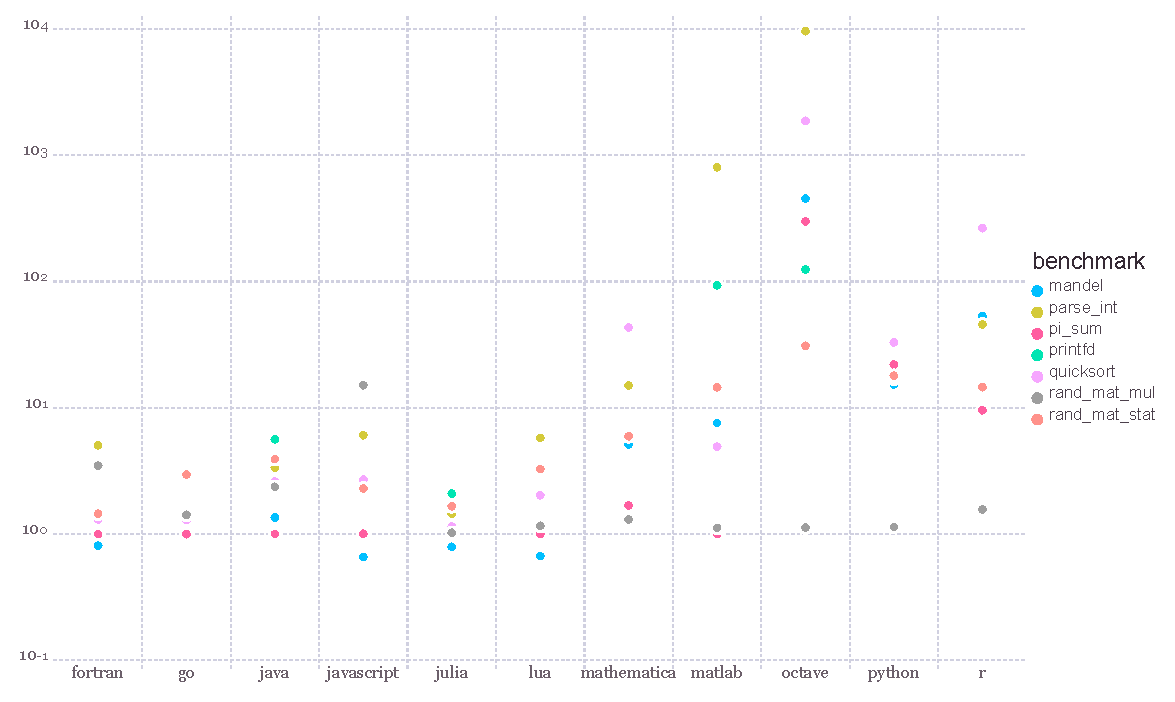
\includegraphics[width=1\textwidth]{juliabenchmarks}
    \end{figure}%
    \let\thefootnote\relax\footnotetext{\href{http://julialang.org/benchmarks}{\tt julialang.org/benchmarks}}
\end{frame}

\subsection{Programação Concorrente, Paralela e Distribuída em Julia}

\begin{frame}[fragile]
    \frametitle{Programação Paralela e Distribuída em Julia}
    O paralelismo em Julia é feito através da troca de mensagens
    entre processos:
    \begin{itemize}
        \item Diferente do MPI, o usuário controla
            explicitamente \alert{apenas um processo}
            \pause
        \item \alert{Remote calls}: executam uma \alert{expressão} em
            outro processo e devolvem uma referência remota (\alert{RemoteRef})
            \pause
        \item \alert{Remote references}: Contém uma referência para objetos
            em \alert{outros processos}
            \pause
        \item \alert{Threading}: \href{https://github.com/JuliaLang/julia/pull/13410}{Pull request \#13410}
    \end{itemize}
    \let\thefootnote\relax\footnotetext{\href{http://docs.julialang.org/en/stable/stdlib/parallel}{\tt docs.julialang.org/en/stable/stdlib/parallel}}
    \let\thefootnote\relax\footnotetext{\href{http://docs.julialang.org/en/stable/manual/parallel-computing}{\tt docs.julialang.org/en/stable/manual/parallel-computing}}
\end{frame}

\begin{frame}[fragile]
    \frametitle{Programação Paralela e Distribuída em Julia}
    Um \alert{ClusterManager} é responsável por:
    \begin{itemize}
        \item Lançar processos (\alert{workers}) Julia numa rede
            \pause
        \item Gerenciar \alert{eventos} e \alert{comunicação}
            entre processos
            \pause
        \item Gerenciar o \alert{transporte} de dados
    \end{itemize}
    \pause
    Algumas funções e objetos disponíveis:
    \begin{lstlisting}
LocalManager::ClusterManager
SSHManager::ClusterManager

addprocs()
rmprocs()
procs()
    \end{lstlisting}
    \let\thefootnote\relax\footnotetext{\href{http://docs.julialang.org/en/stable/stdlib/parallel}{\tt docs.julialang.org/en/stable/stdlib/parallel}}
    \let\thefootnote\relax\footnotetext{\href{http://docs.julialang.org/en/stable/manual/parallel-computing}{\tt docs.julialang.org/en/stable/manual/parallel-computing}}
\end{frame}

\begin{frame}[fragile]
    \frametitle{Programação Paralela e Distribuída em Julia}
    Chamadas de funções:

    \begin{lstlisting}
Task(func)
remotecall(id, func, args..)
remotecall_fetch(id, func, args..)
remotecall_wait(id, func, args..)
    \end{lstlisting}
    \pause
    \begin{lstlisting}
put!(RemoteRef, value)
take!(RemoteRef)
    \end{lstlisting}
    \pause
    \begin{lstlisting}
fetch(RemoteRef)
wait(RemoteRef)
    \end{lstlisting}
    \pause
    \begin{lstlisting}
produce(value)
consume(Task, values..)
    \end{lstlisting}
    \let\thefootnote\relax\footnotetext{\href{http://docs.julialang.org/en/stable/stdlib/parallel}{\tt docs.julialang.org/en/stable/stdlib/parallel}}
    \let\thefootnote\relax\footnotetext{\href{http://docs.julialang.org/en/stable/manual/parallel-computing}{\tt docs.julialang.org/en/stable/manual/parallel-computing}}
\end{frame}

\begin{frame}[fragile]
    \frametitle{Programação Paralela e Distribuída em Julia}
    Usando macros:
    \begin{lstlisting}
@task()
@spawn()
@spawnat()
    \end{lstlisting}
    \pause
    \begin{lstlisting}
@fetch()     = fetch(@spawn expr)
@fetchfrom() = fetch(@spawnat p expr)
    \end{lstlisting}
    \pause
    \begin{lstlisting}
@async()
@sync()

@parallel()
@everywhere()
    \end{lstlisting}
    \let\thefootnote\relax\footnotetext{\href{http://docs.julialang.org/en/stable/stdlib/parallel}{\tt docs.julialang.org/en/stable/stdlib/parallel}}
    \let\thefootnote\relax\footnotetext{\href{http://docs.julialang.org/en/stable/manual/parallel-computing}{\tt docs.julialang.org/en/stable/manual/parallel-computing}}
\end{frame}

\subsection{Detalhes de Implementação}

\begin{frame}[fragile]
    \frametitle{StochasticSearch.jl}
    \begin{figure}[H]
        \centering
        
\includegraphics[width=.7\textwidth]{stochasticsearchlogo}
    \end{figure}%
    \begin{itemize}
        \item Pacote para \alert{Busca Estocástica Local}
        \item \alert{Independente} de domínio
        \item \alert{Conjuntos} de técnicas de busca
            \pause
        \item Técnicas de execução \alert{independente}
        \item Técnicas de busca \alert{modulares}
            \pause
        \item Execução \alert{paralela} e \alert{distribuída}
            \pause
        \item Maior \alert{controle} do fluxo de execução
    \end{itemize}
\end{frame}

\begin{frame}[fragile]
    \frametitle{StochasticSearch.jl}
    \begin{itemize}
        \item Código sob Licença MIT:

            \href{http://github.com/phrb/StochasticSearch.jl}{\tt github.com/phrb/StochasticSearch.jl}
        \item Disponível no \alert{repositório oficial}:
            \begin{lstlisting}[language=bash]
julia> Pkg.add("StochastichSearch")
            \end{lstlisting}
            \pause
        \item Testes de Unidade: \alert{97\%} de cobertura:

                \href{https://coveralls.io/github/phrb/StochasticSearch.jl}{\tt coveralls.io/github/phrb/StochasticSearch.jl}
        \item Integração Contínua (\alert{TravisCI}):

            \href{https://travis-ci.org/phrb/StochasticSearch.jl}{\tt travis-ci.org/phrb/StochasticSearch.jl}
    \end{itemize}
\end{frame}

\subsection{Busca Estocástica Local}

\begin{frame}[fragile]
    \frametitle{Busca Estocástica Local: Composição}
    Blocos de construção:
    \begin{itemize}
        \item First Improvement
        \item Probabilistic Improvement
        \item Greedy Construction
        \item Random Walk
            \pause
        \item \alert{TODO}: Best Improvement
    \end{itemize}
\end{frame}

\begin{frame}[fragile]
    \frametitle{Busca Estocástica Local: Composição}
    Técnicas de busca usando os blocos:

    \alert{DONE}:
    \begin{itemize}
        \item Iterative First Improvement
        \item Iterative Probabilistic Improvement
        \item Iterative Greedy Construction
        \item Randomized First Improvement
        \item Simulated Annealing
    \end{itemize}
    \pause

    \alert{TODO}:
    \begin{itemize}
        \item Randomized Best Improvement
        \item Iterative Probabilistic Improvement
        \item Iterated Local Search
        \item Tabu Search
        \item Ant Colony Optimization
        \item Particle Swarm Optimization
        \item ...
    \end{itemize}
\end{frame}

\subsection{Comparando com o OpenTuner}

\begin{frame}[fragile]
    \frametitle{Comparações com o OpenTuner: Fluxo de Execução}
    Obtenção de um resultado no OpenTuner, simplificadamente:
    \begin{figure}[H]
        \centering
        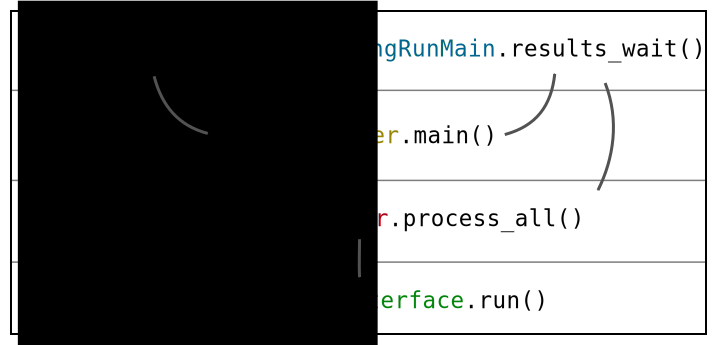
\includegraphics[width=.9\textwidth]{opentunerflow_simple}
    \end{figure}%
\end{frame}

\begin{frame}[fragile]
    \frametitle{Comparações com o OpenTuner: Fluxo de Execução}
    Obtenção de um resultado no StochasticSearch.jl, simplificadamente:
    \begin{figure}[H]
        \centering
        \includegraphics[width=.55\textwidth]{stochasticsearchflow_simple}
    \end{figure}%
\end{frame}

\begin{frame}[fragile]
    \frametitle{Comparações com o OpenTuner: Esforço de Implementação}
    \begin{figure}[H]
        \centering
        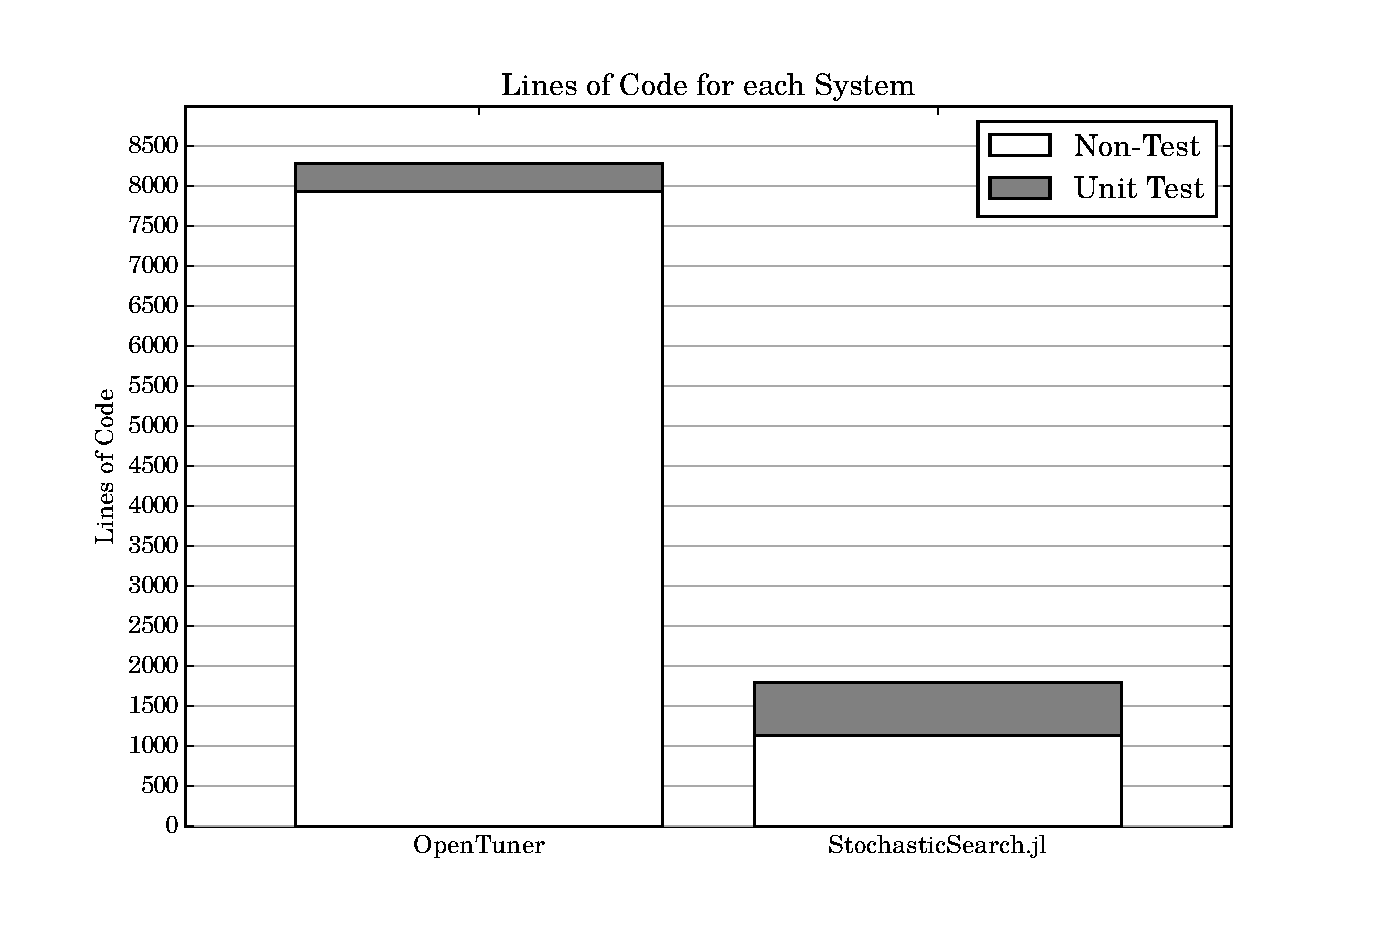
\includegraphics[width=1\textwidth]{loc_comparison}
    \end{figure}%
\end{frame}

\begin{frame}[fragile]
    \frametitle{Comparações: Travelling Salesperson Problem}
    \begin{figure}[H]
        \centering
        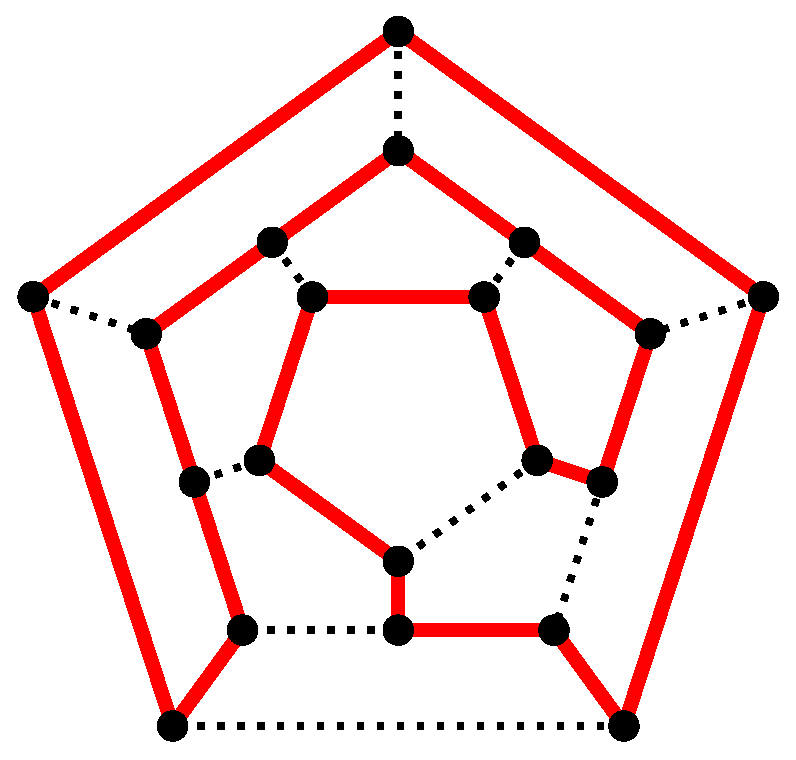
\includegraphics[width=.28\textwidth]{hamiltonianpath}
    \end{figure}%
    Comparação do desempenho de \alert{autotuners} que resolvem
    instâncias\footnotemark{} do TSP, implementados com o OpenTuner e 
    com o StochasticSearch.jl.
    \pause

    As soluções são representadas por \alert{permutações} das cidades.

    \pause
    Disponível em:
    \href{https://github.com/phrb/stochasticsearch-docs}{\tt github.com/phrb/stochasticsearch-docs}

    \footnotetext{TSPLIB: \url{http://goo.gl/8ZZXi2}}
\end{frame}

\begin{frame}[fragile]
    \frametitle{Comparações: Desempenho TSP (532 Cidades)}
    \begin{figure}[H]
        \centering
        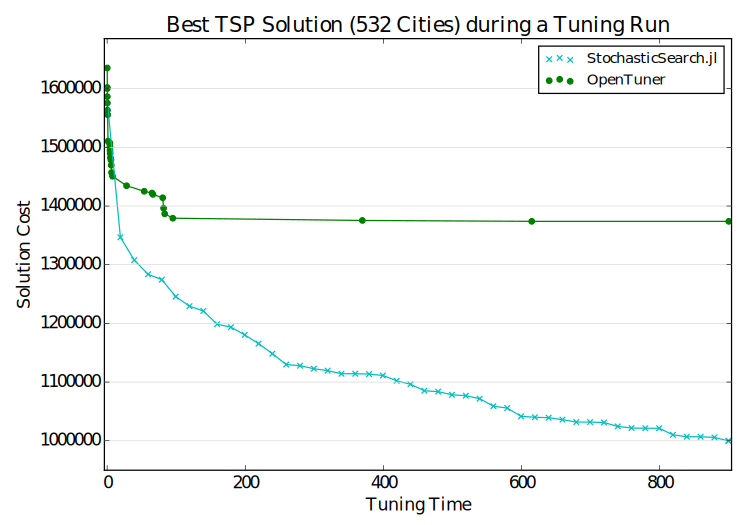
\includegraphics[width=1\textwidth]{att532_15min_best_comparison}
    \end{figure}%
\end{frame}

\begin{frame}[fragile]
    \frametitle{Comparações: Desempenho TSP (532 Cidades)}
    \begin{figure}[H]
        \centering
        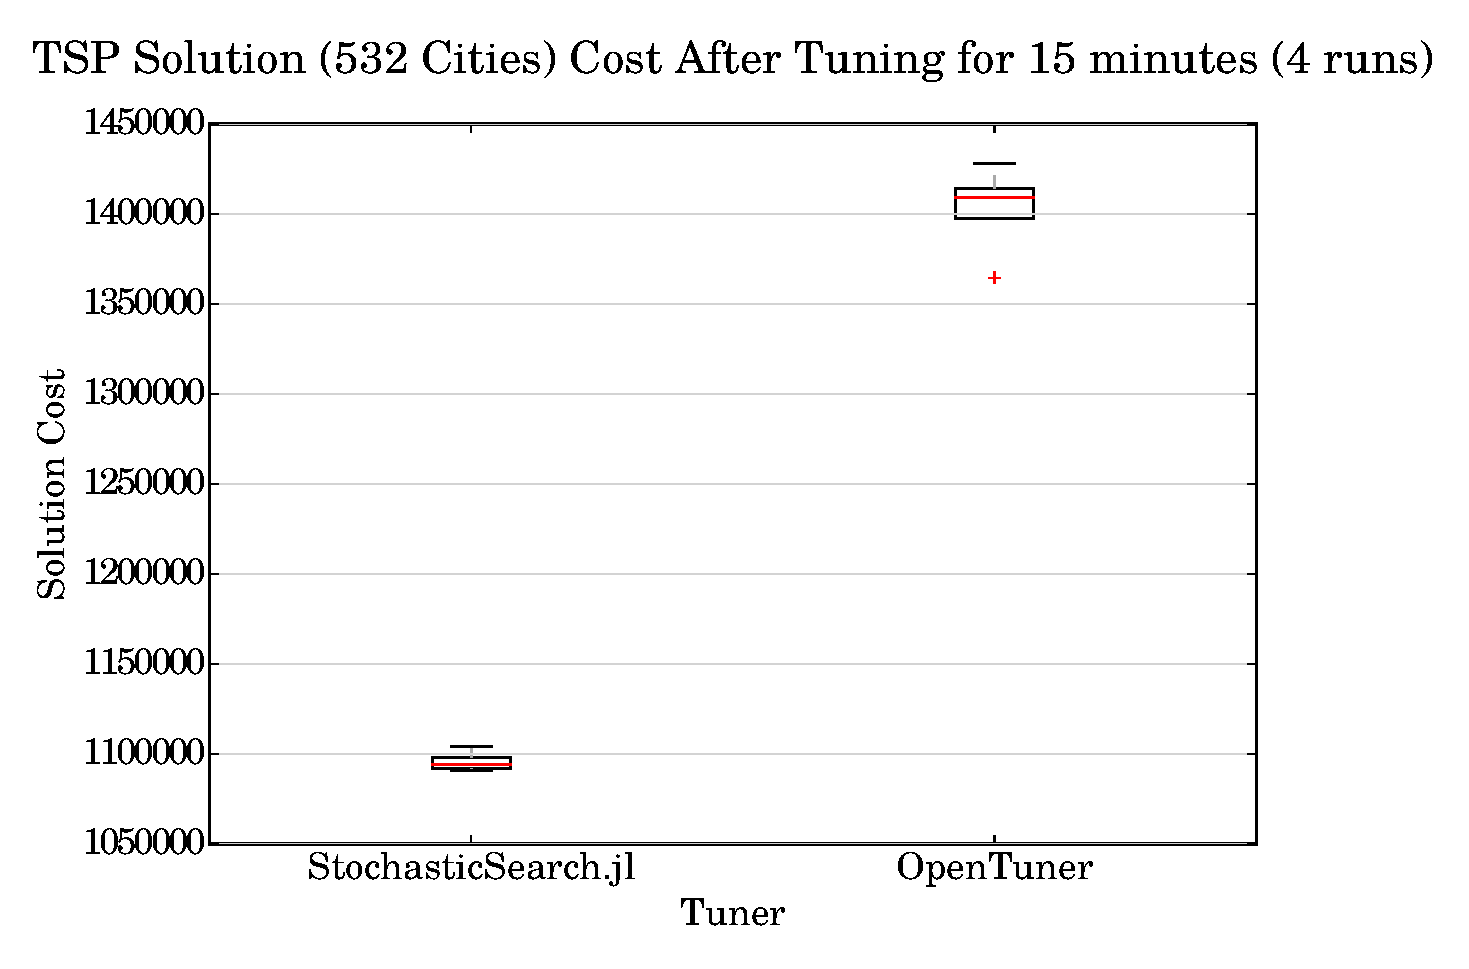
\includegraphics[width=1\textwidth]{att532_15min_comparison}
    \end{figure}%
\end{frame}

\begin{frame}[fragile]
    \frametitle{Comparações: Desempenho TSP (85900 Cidades)}
    \begin{figure}[H]
        \centering
        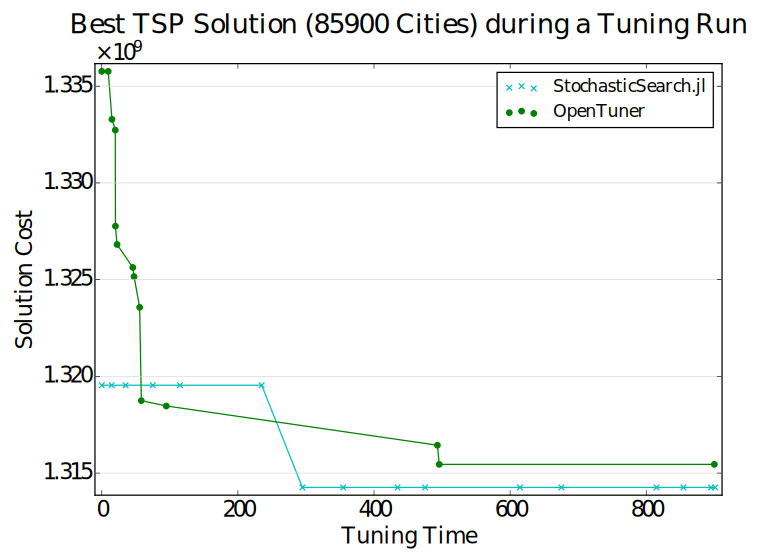
\includegraphics[width=1\textwidth]{pla85900_15min_best_comparison}
    \end{figure}%
\end{frame}

\begin{frame}[fragile]
    \frametitle{Comparações: Desempenho TSP (85900 Cidades)}
    \begin{figure}[H]
        \centering
        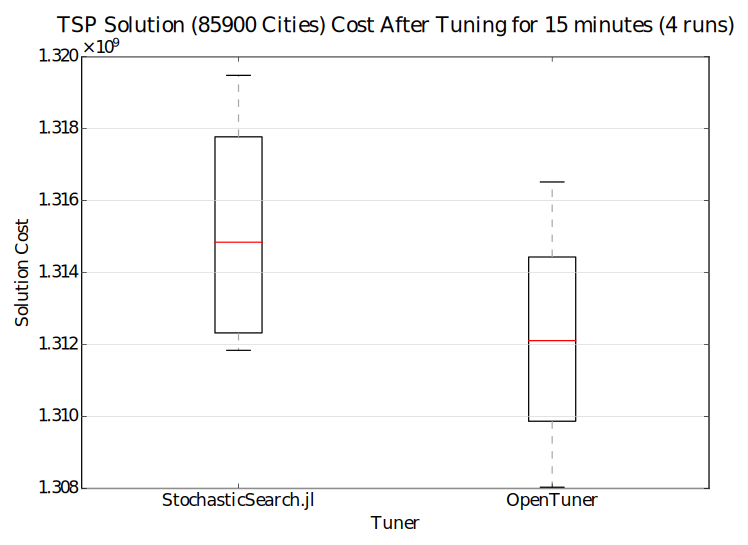
\includegraphics[width=1\textwidth]{pla85900_15min_comparison}
    \end{figure}%
\end{frame}

\section{Trabalhos Futuros}

\begin{frame}[fragile]
    \frametitle{Trabalhos Futuros}
    \begin{itemize}
        \item Implementar Busca Estocástica Local no \alert{OpenTuner}
            \pause
        \item \alert{Adicionar}, \alert{remover} e \alert{modificar} técnicas
            de busca e parâmetros em \alert{tempo de execução}
            \pause
        \item Implementar \alert{ClusterManagers} para \alert{GPUs} e \alert{Nuvem}
            \pause
        \item Parâmetros de compilação \alert{CUDA}
        \item Resolvedores \alert{SAT}
            \pause
        \item Experimentos com \alert{domínios diferentes}
        \item Experimentos com \alert{execução distribuída}
            \pause
        \item \alert{Aumentar} a cobertura de testes
            \pause
        \item Implementar técnicas de busca mais \lq{}\lq{}\alert{poderosas}\rq{}\rq{}
    \end{itemize}
\end{frame}

\begin{frame}[fragile]
    \frametitle{Trabalhos Futuros}
    Responder às perguntas:
    \begin{itemize}
        \item \alert{RQ1}: Técnicas de busca estocástica apresentam
            alguma vantagem em relação a outras técnicas de autotuning?
            \pause
        \item \alert{RQ2\textbf{a}}: Como utilizar programação paralela e
            distribuída para melhorar o desempenho de autotuners?
            \pause
        \item \alert{RQ2\textbf{b}}: Para quais domínios de problema isso é
            vantajoso?
    \end{itemize}
\end{frame}

\plain{Obrigado!}

\maketitle

\end{document}
